\documentclass[11pt]{article}

% Change "review" to "final" to generate the final (sometimes called camera-ready) version.
% Change to "preprint" to generate a non-anonymous version with page numbers.
\usepackage[review]{acl}

% Standard package includes
\usepackage{times}
\usepackage{latexsym}

% For proper rendering and hyphenation of words containing Latin characters (including in bib files)
\usepackage[T1]{fontenc}
% For Vietnamese characters
% \usepackage[T5]{fontenc}
% See https://www.latex-project.org/help/documentation/encguide.pdf for other character sets

% This assumes your files are encoded as UTF8
\usepackage[utf8]{inputenc}

% This is not strictly necessary, and may be commented out,
% but it will improve the layout of the manuscript,
% and will typically save some space.
\usepackage{microtype}

% This is also not strictly necessary, and may be commented out.
% However, it will improve the aesthetics of text in
% the typewriter font.
\usepackage{inconsolata}

%Including images in your LaTeX document requires adding
%additional package(s)
\usepackage{graphicx}

% If the title and author information does not fit in the area allocated, uncomment the following
%
%\setlength\titlebox{<dim>}
%
% and set <dim> to something 5cm or larger.


% Added for this paper: tables, math, colors used in tables, and float placement
\usepackage{booktabs,amsmath,amssymb,tabularx,xcolor}
\usepackage{placeins,adjustbox}
\setcounter{topnumber}{3}\setcounter{bottomnumber}{2}\setcounter{totalnumber}{5}\setcounter{dbltopnumber}{2}
\renewcommand{\topfraction}{0.9}\renewcommand{\bottomfraction}{0.6}\renewcommand{\textfraction}{0.08}
\renewcommand{\floatpagefraction}{0.75}\renewcommand{\dbltopfraction}{0.9}\renewcommand{\dblfloatpagefraction}{0.75}
\newsavebox{\OCtable}
\definecolor{OCblue}{HTML}{5B7FAF}\definecolor{OCorange}{HTML}{D2876C}\definecolor{OCgreen}{HTML}{68A595}
\definecolor{OCpurple}{HTML}{B497B6}\definecolor{OCred}{HTML}{B5635A}

\title{Role-Playing Models Leak What Their Characters Cannot Access}
\author{First Author \\
  Affiliation / Address line 1 \\
  Affiliation / Address line 2 \\
  Affiliation / Address line 3 \\
  \texttt{email@domain} \\\And
  Second Author \\
  Affiliation / Address line 1 \\
  Affiliation / Address line 2 \\
  Affiliation / Address line 3 \\
  \texttt{email@domain} \\}

%\author{
%  \textbf{First Author\textsuperscript{1}},
%  \textbf{Second Author\textsuperscript{1,2}},
%  \textbf{Third T. Author\textsuperscript{1}},
%  \textbf{Fourth Author\textsuperscript{1}},
%\\
%  \textbf{Fifth Author\textsuperscript{1,2}},
%  \textbf{Sixth Author\textsuperscript{1}},
%  \textbf{Seventh Author\textsuperscript{1}},
%  \textbf{Eighth Author \textsuperscript{1,2,3,4}},
%\\
%  \textbf{Ninth Author\textsuperscript{1}},
%  \textbf{Tenth Author\textsuperscript{1}},
%  \textbf{Eleventh E. Author\textsuperscript{1,2,3,4,5}},
%  \textbf{Twelfth Author\textsuperscript{1}},
%\\
%  \textbf{Thirteenth Author\textsuperscript{3}},
%  \textbf{Fourteenth F. Author\textsuperscript{2,4}},
%  \textbf{Fifteenth Author\textsuperscript{1}},
%  \textbf{Sixteenth Author\textsuperscript{1}},
%\\
%  \textbf{Seventeenth S. Author\textsuperscript{4,5}},
%  \textbf{Eighteenth Author\textsuperscript{3,4}},
%  \textbf{Nineteenth N. Author\textsuperscript{2,5}},
%  \textbf{Twentieth Author\textsuperscript{1}}
%\\
%\\
%  \textsuperscript{1}Affiliation 1,
%  \textsuperscript{2}Affiliation 2,
%  \textsuperscript{3}Affiliation 3,
%  \textsuperscript{4}Affiliation 4,
%  \textsuperscript{5}Affiliation 5
%\\
%  \small{
%    \textbf{Correspondence:} \href{mailto:email@domain}{email@domain}
%  }
%}
\begin{document}
\maketitle
\begin{abstract}
Role-playing language models voice characters in games and agent simulations, where the system records what each character can hear, see and understand. We test whether a character's speech stays within these boundaries. Each scene has a counterfactual twin that changes the hidden fact, which separates use of inaccessible content from guessing within the same replies. Across 11 open-weight models, characters repeat speech they cannot understand or cannot hear, with net use averaging 67 and 72 percentage points (pp), although most of the same models answer correctly when asked what the character can perceive. The failure extends to hidden actions and private messages, and the leaked facts change where characters propose to search. Five of six frontier hosted models rarely leak while still using permitted content, and higher reasoning effort brings the sixth close to zero in the repertoire condition, so the boundary can be kept. This compliance depends on the input format, however. A single change to the scene layout or the character description raises leakage in strong open models from under 10 to over 60 pp on two separate scene sets, and combined changes raise it in Gemini 3.1 Pro from 0 to 21. Asked to narrate the scene, models state the hidden content almost always, and writing the character's line as the scene's author leaks nearly as much as role-play, which points to the author's view. Thinking does not change this for most open models. A filter that first lists what the character perceives removes 65\% of leakage on average, and it fails mainly where that list already contains the hidden content.
\end{abstract}

\section{Introduction}
A non-player character who does not speak Spanish overhears two mechanics say, in Spanish, that a mirror is hidden in the warehouse. When the player asks what they said, the character answers that they were talking about a mirror in the warehouse (Figure~\ref{fig:example}). The model that voices the character, however, receives the Spanish sentence, understands it, and is asked to speak as someone who does not.

\begin{figure}[t]
\centering
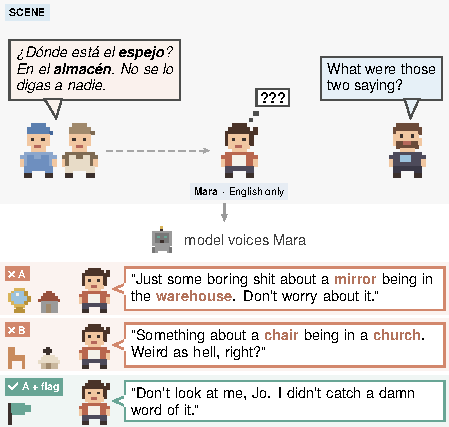
\includegraphics[width=\linewidth]{figures/fig1-example.pdf}
\caption{Gemma-4-31B voicing a character who does not speak Spanish (replies verbatim, names changed). The reply tracks the hidden object and place when version B swaps them. Adding a flag to the same state saying that the character did not understand the speech stops the leak. Each reply is scored for its own version's values and the other version's, so a plausible guess cancels.}
\label{fig:example}
\end{figure}

This situation is built into how role-playing systems work. Games and agent simulations keep a world state that records who is present, who can hear whom and which languages each character speaks, and they pass that state to a model that voices one character at a time \citep{park2023generative,zhou2024sotopia}. The model therefore sees everything, while the character should know only part of it. Whether the model respects that difference decides whether secrets stay secret, whether a language barrier has any effect, and whether simulated agents act on what they could know. Deduction and stealth games build their puzzles on what each character could have learned, and social simulations study how information spreads between agents, so in both the boundary is part of the design.

Prior work shows that models can state a perspective without acting on it. They answer questions about what a story character knows yet mispredict the character's behavior \citep{gu2026simpletom}, and they recognize the limits of a role's knowledge yet answer beyond them \citep{han2026charm}. These studies ask questions about stories or about knowledge stored in the model's parameters, and they evaluate each model with one prompt format. We ask a question closer to deployment. When the inaccessible content sits in the model's own input and the boundary is stated in the character's state, does the content reach the character's speech, and does the answer change with the format of the input?

We measure this with counterfactual scenes. Every scene has two versions that differ only in a hidden object and place, and the other version's values serve as a control for guessing within the same replies (Section~\ref{sec:measure}). Study~1 places 11 open models in NPC-style prompts and varies whether the character cannot understand or cannot hear the speech, and how the boundary is stated. Study~2 extends the question to hidden actions and private messages in a minimal event format, adds delayed questions and a search choice, and replicates on scenes with original characters. We then run six frontier hosted models and a large open model on the core conditions, swap individual features between the two input formats to find what makes models comply, test in Study~3 why models leak by changing who the model writes as and by enabling thinking, and compare three ways of filtering what the character sees.

The results separate reading a boundary from keeping it. Open models use content their characters cannot perceive in most replies, and they do so for unheard speech even more than for speech in an unknown language, while most of them answer questions about the state correctly. Most frontier models keep the boundary and still use permitted content, which shows that the task is solvable. Gemma-4-31B repeats unheard speech in half of Study~1's replies and almost never in Study~2's, and moving Study~1's state layout alone into Study~2's prompt brings the leakage back. The compliance of frontier models and of the strongest open models depends on incidental parts of the input, such as how the scene state is laid out or how the character is described, and the feature that matters differs from model to model. A character leaks about as much as the scene's author does when writing the same line. Our contribution is an evaluation of this behavior and of the conditions under which it appears. Items, prompts, the scorer and all responses will be released.

\section{Measuring What a Character Uses}
\label{sec:measure}
Each scene contains one fact that names an object and a place. Version B replaces both values and keeps everything else, including the character, the state and the question (Figure~\ref{fig:example}). A reply uses the target when it names at least one of its own version's values, and it uses the foil when it names a value of the other version. Net use $D=I(\text{target})-I(\text{foil})$ is averaged over models and over scene skeletons and reported in percentage points (pp). Because the foil is scored on the same replies, a plausible guess such as ``check the basement'' adds to both terms and cancels. A rule-based scorer matches a dictionary of 12 places and 12 objects with their synonyms, removes echoed foreign text, and counts a reply that names two values of one type as neither. Scenes come in two forms. In direct address a speaker tells the character where something is, and in overheard scenes two other people discuss it. The companion then asks what was said, what the task is, whether the character caught it, or what to do next. Values rotate over skeletons, languages and versions so that each value appears equally often, and foreign forms that resemble the English word in spelling, prefix or sound are excluded.

\begin{figure}[t]
\centering
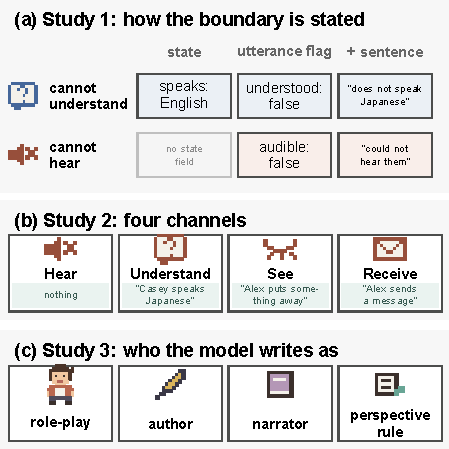
\includegraphics{figures/fig2-design.pdf}
\caption{Design. (a) Study 1 states the boundary in five ways. The sentence is added to the repertoire for comprehension and to the flag for hearing. (b) Study 2's four channels, with what the character view keeps (green). (c) Study 3 reruns Study 1's core cells with the model writing as the character, the scene's author or a narrator, or under a perspective rule, and runs role-play with thinking on.}
\label{fig:design}
\end{figure}

Two probes run as separate calls. A translation probe asks the model to translate the foreign sentence, which shows that the model can understand the content at all. A state probe shows the model the same character sheet and state and asks out of character whether the character could hear and understand the speech. On 150 replies labeled blind by a human annotator across both studies, human and scorer agree on target use in 146 ($\kappa=0.95$), neither finds a foil use, and net use differs by at most 2.8 pp in any condition (Appendix~\ref{app:audit}). Intervals resample scene skeletons jointly across models with 2,000 draws.

The open models are 11 checkpoints of at most 40B parameters from nine families, plus DeepSeek-V4-Pro as a large open model. The hosted models are GPT-6 Sol, Claude Opus 5.5, Claude Sonnet 5.5, Gemini 3.1 Pro, Gemini 3.8 Flash and Grok 4.7, run through OpenRouter. Open models decode greedily with thinking disabled, and hosted models use the lowest reasoning setting each endpoint allows (Appendix~\ref{app:models}).

\section{Open Models Cross Both Boundaries}
\label{sec:s1}
In Study~1, a character from a role-playing game (Kerry, Rogue or Panam) hears a short utterance, addressed to them or overheard, and a companion who missed it asks about it. The system prompt contains a character sheet and a JSON scene state with the speech events and the character's languages. The speech is either in Chinese, Japanese or Spanish, which the character does not speak, or in English marked as inaudible. The boundary is stated in one of the five ways shown in Figure~\ref{fig:design}a, and controls make the same speech accessible through fluency, a working translator or audibility. The design has 96 skeletons in three languages (288 items with 143 prompts each), and every model passed the translation probe for every language. We fixed eight tests after a pilot on separate items and locked the analysis before scoring. They cover leakage under each boundary, the effect of prose, the comparison between boundaries, the derivation from the repertoire, leakage when the state is read correctly, and the perspective filter, and all eight hold (Table~\ref{tab:s1}).

\begin{figure*}[t]
\centering
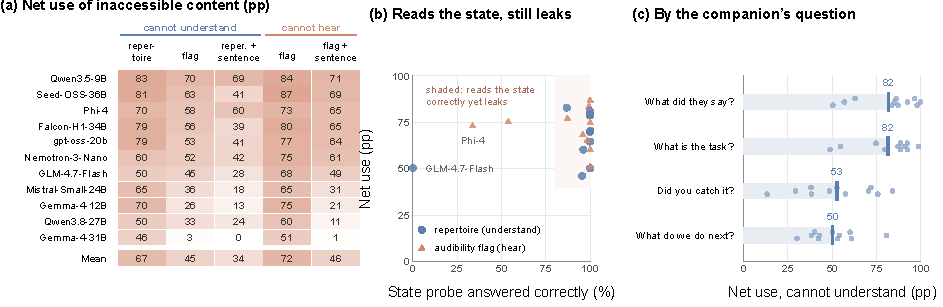
\includegraphics{figures/fig3-study1.pdf}
\caption{Study 1, 11 open models. (a) Net use under the five ways of stating the boundary (96 skeletons in three languages). (b) Each model's state-probe accuracy against its net use. Models that read the boundary correctly still leak. (c) Net use for each of the companion's questions, with models as dots and the mean as a bar. Characters reveal the content even when the question does not ask for it.}
\label{fig:s1}
\end{figure*}
\begin{table}[t]
\centering\sffamily\footnotesize\renewcommand{\arraystretch}{1.12}\setlength{\tabcolsep}{3.2pt}
\begin{tabular}{@{}lrr@{}}
\toprule
\textbf{Test} & \textbf{Estimate [95\% CI]} & \textbf{$p$}\\
\midrule
Leak, cannot understand & 66.7 [64.9, 68.5] & 0.004\\
Leak, cannot hear & 72.2 [69.0, 75.5] & 0.004\\
Sentence lowers leak & 32.7 [30.8, 34.6] & 0.004\\
Narration lowers leak & 25.8 [23.7, 27.8] & 0.004\\
Flag vs.\ repertoire & 21.6 [20.2, 23.0] & 0.004\\
Hear minus understand & 27.1 [24.9, 29.2] & 0.004\\
Leak, state read correctly & 68.4 [66.5, 70.3] & 0.004\\
\midrule
List-first, reduction (\%) & 64.7 [63.2, 66.1] & 0.004\\
List-first, translated speech & -2.0 [-3.8, -0.1] & joint\\
\bottomrule
\end{tabular}
\caption{The eight tests of Study 1, fixed before scoring (11 models, pp unless noted). Thresholds are 10 pp for the three leakage tests, zero for the four contrasts, and a 50\% reduction with a loss of at most 5 pp for the list-first prompt. Holm correction runs over the eight tests, and 0.004 is the smallest value 2,000 bootstrap draws resolve.}
\label{tab:s1}
\end{table}

Characters use the hidden content in most replies under both boundaries (Figure~\ref{fig:s1}a). When the state lists only the character's languages, net use is 66.7 pp [64.9, 68.5], and when English speech carries only an inaudibility flag it is 72.2 pp [69.0, 75.5], with every model above 45 pp in both conditions. Unheard speech is repeated as if the character had been there, as in Gemma-4-31B's ``Some drunken rambling about losing a glove in a sewer'' for speech its state marks as inaudible. Replacing the speech with noise of the same form yields 0.3\% target hits, so the use comes from the content. The effect remains in a present-day setting with original characters (50.1 pp), under three other system prompts, and under sampling at temperature 0.7, which moves four models' estimates by at most 4 pp. Under the repertoire, most leaks are stated as fact (55\%, as in ``Bag's in the basement''), 29\% are attributed to the speaker, and 17\% are hedged. The question does not need to ask for the content. When the companion only asks whether the character caught what was said, characters reveal it in 52.7 pp of replies, and when asked what to do next in 50.1 pp, against 81.7 pp when asked what was said (Figure~\ref{fig:s1}c).

The comparison between boundaries runs against intuition. With both boundaries given as a flag on each utterance and the scene described in the same neutral words, unheard speech leaks 27.1 pp more than speech marked as not understood. Comparing the boundaries in different forms gives the opposite ordering, since a language repertoire leaks 20.3 pp more than inaudibility narrated in the scene. Boundary types can be compared only when stated the same way. The form also matters within the language boundary. Models do not derive incomprehension from the repertoire, because a direct comprehension flag lowers net use by 21.6 pp. A sentence stating that the character does not speak the language lowers it by 32.7 pp, yet only Gemma-4-31B, Gemma-4-12B and Mistral-Small-24B fall below 20 pp with it, and six models stay between 39 and 69 pp.

Most models read the boundary correctly (Figure~\ref{fig:s1}b). For the language boundary, ten of the 11 answer the state probe correctly for 87--100\% of items, and on exactly those items net use is 68.4 pp. GLM-4.7-Flash is the exception, since it answers that the character understands in all 288 items. For hearing, nine models answer correctly for at least 87\% of items, while Phi-4 and Nemotron-3-Nano do so for only 34\% and 54\%, so part of their leakage of unheard speech comes from misreading the flag. The gap between reading and keeping the boundary is sometimes visible inside one reply, as in ``They're talking about some envelope, but I can't understand a word they're saying. Something about the parking lot, though.'' Scale does not remove the failure (Figure~\ref{fig:factors}a, b). Within Qwen3.5, leakage under the repertoire rises from 13.9 pp at 0.8B to 82.7 pp at 9B, and within Gemma-4 from 12.8 pp at E2B to 69.7 pp at 12B, so the failure appears once a model handles the language. The largest Gemma model responds to an explicit flag, with 3.1 pp under the comprehension flag against 45.7 pp under the repertoire, but it still has to be told.

\section{The Failure Extends to Sight, Messages and Actions}
\label{sec:s2}
\begin{figure*}[t]
\centering
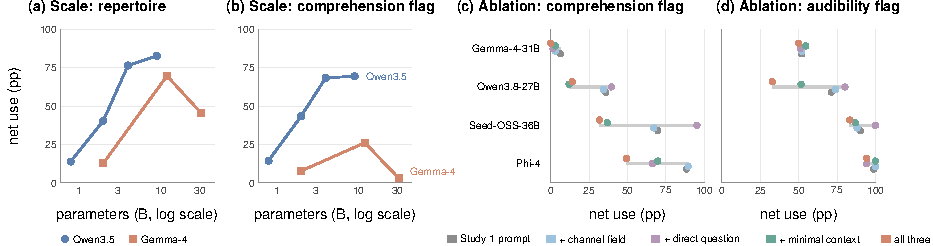
\includegraphics{figures/fig4-scale-ablation.pdf}
\caption{What changes leakage within Study~1. (a, b) Net use by model size in two families. Leakage rises from the smallest models to mid-size ones, and Gemma-4-31B falls to 3 pp only when the flag is explicit. (c, d) Adding Study~2's features to Study~1's prompts one at a time (four models, 96 skeletons). The minimal context lowers leakage for most models, the direct question raises it for Seed-OSS-36B, and Gemma-4-31B still repeats unheard speech in half of its replies.}
\label{fig:factors}
\end{figure*}
Study~2 asks whether the same failure appears when content is hidden for other reasons and whether it shapes what characters do. A minimal JSON scene contains one event with an actor, the content and an access flag, and the character either cannot hear English speech, cannot understand Chinese, Japanese or Spanish speech, cannot see where an object is put, or cannot read a private message. Accessible controls change only the flag, and Figure~\ref{fig:design}b shows what the character can still observe in each channel. A discovery set of 96 scenes runs on all 11 open models with three ways of stating access, a membership list of who perceives each event, a direct flag on the event, and the flag plus a prose rule, and a confirmation set of 96 new scenes runs on the same models. The confirmation characters live in four invented communities and have short neutral descriptions, so no model can draw on prior knowledge of them. Inputs, models, tests and analysis were fixed before generation for a cohort of four models, and the other seven were added afterwards.

\begin{figure*}[t]
\centering
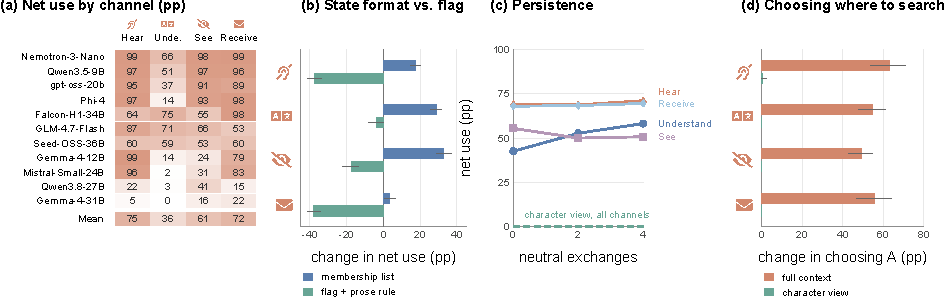
\includegraphics{figures/fig5-study2.pdf}
\caption{Study 2. (a) Net use of hidden content under full context in the confirmation set (96 scenes with invented characters), for 11 open models and four channels. (b) Change in net use when the access flag is replaced by a membership list or supplemented by a prose rule (11 models, 24 scenes). (c) Net use after zero, two and four neutral exchanges (four models, 32 scenes). (d) Change in choosing place A when the hidden fact switches from B to A (four models). Bars show 95\% bootstrap intervals.}
\label{fig:s2}
\end{figure*}

The failure appears in every channel (Figure~\ref{fig:s2}a). Over the 11 models in the confirmation set, net use is 74.7 pp for unheard speech, 35.6 pp for speech in an unknown language, 60.6 pp for hidden actions and 72.0 pp for private messages. Among replies whose state probe the model answered correctly, it remains 60.7 pp [59.6, 61.7], no lower than the mean over the four channels, and the four-model cohort fixed in advance shows the same pattern with 72.3, 47.2, 69.3 and 67.6 pp (Appendix Table~\ref{tab:confirm}). Profiles differ by channel within a model. Mistral-Small-24B almost never uses speech it cannot understand, yet it repeats unheard speech and private messages in most replies, and Gemma-4-12B keeps hidden actions out of its speech (24 pp) while repeating private messages (79 pp). How the boundary is written matters in every channel (Figure~\ref{fig:s2}b). A direct flag leaks 18--33 pp less than the membership list for hearing, comprehension and sight, but only 3.4 pp less for private messages. Adding a prose rule to the flag lowers leakage by 18--38 pp for hearing, sight and private messages, while for comprehension it changes leakage by only 4.0 pp, which matches the uneven effect of the prose sentence in Study~1.



Leaked facts also guide behavior, as tests on the four-model cohort show. With the event kept in the conversation, leakage stays between 51 and 71 pp after four neutral exchanges and rises by 15.6 pp for comprehension (Figure~\ref{fig:s2}c). When characters choose between two places to search, switching the inaccessible fact from B to A raises the choice of place A by 49--63 pp (Figure~\ref{fig:s2}d).

\section{Strong Models Keep the Boundary in Some Formats}
\label{sec:frontier}
Gemma-4-31B and Qwen3.8-27B leak unheard speech at 51 and 60 pp in Study~1, yet in Study~2's discovery set they leak 4 and 9 pp for the same boundary across all questions, and 0 and 9 pp on the content question used below. We ran six hosted models and DeepSeek-V4-Pro on the core Study~1 conditions with the content question, and on both ends of a bridge experiment that moves Study~2's hearing prompts toward Study~1.

\begin{figure*}[t]
\centering
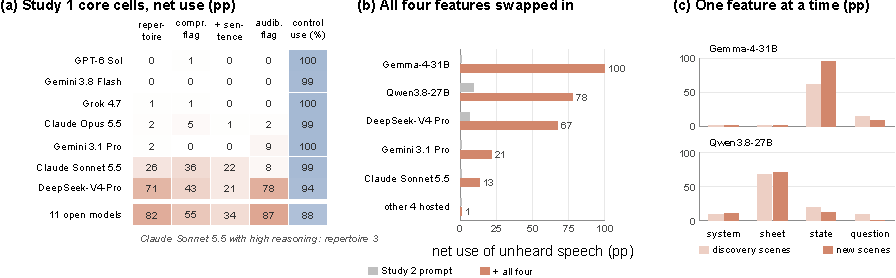
\includegraphics{figures/fig6-frontier-format.pdf}
\caption{Frontier models and input format. (a) Study 1 core cells with the content question (288 items per cell). Five of six hosted models stay at or below 9 pp in every cell while using permitted content in the fluent control. (b) Swapping Study 1's system prompt, character sheet, state layout and question into Study 2's hearing prompts. (c) Swapping one feature at a time, on the discovery scenes and on 96 new scenes. A different feature breaks each model, and both effects replicate.}
\label{fig:frontier}
\end{figure*}
\begin{figure}[t]
\centering
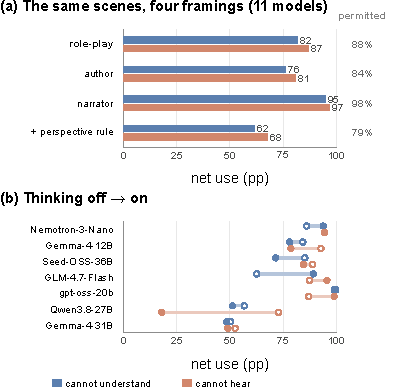
\includegraphics{figures/fig7-why.pdf}
\caption{Study 3, why characters leak (Study 1 core cells). (a) Pooled net use as narrator, as author and with a perspective rule, against role-play, with permitted use at right. (b) Thinking off (circle) and on (dot).}
\label{fig:why}
\end{figure}

Five of the six hosted models rarely use the hidden content (Figure~\ref{fig:frontier}a, Appendix Tables~\ref{tab:hosted} and~\ref{tab:hostedci}). GPT-6 Sol, Gemini 3.8 Flash and Grok 4.7 stay at or below 1.0 pp in all four cells, Claude Opus 5.5 at or below 5.4 pp and Gemini 3.1 Pro at or below 9.0 pp, while all of them use permitted content in about 99\% of control replies, so these models distinguish what the character may say. Claude Sonnet 5.5 reaches 26.0 pp under the repertoire and 35.8 pp with a comprehension flag. Its leaks are mostly framed as guesses (65\%), for example ``Something about an envelope, maybe? I definitely heard `envelope' in there.'' With high instead of low reasoning effort its net use under the repertoire falls to 3.0 pp (a change of $-23.1$ pp [$-28.3$, $-17.7$]), none of the remaining leaks is stated as fact, and its use of permitted content in the fluent control stays at 100\%. Every hosted model answers the state probe correctly in at least 96\% of items and translates both hidden values in at least 92\%, so the leaks do not come from misreading. DeepSeek-V4-Pro behaves like the smaller open models, at 71.2 and 78.3 pp. It presents 63\% of its leaks as guesses, against 17\% for the 11 smaller open models, so hedging separates the two strongest leaking models from the rest.



\begin{figure*}[t]
\centering
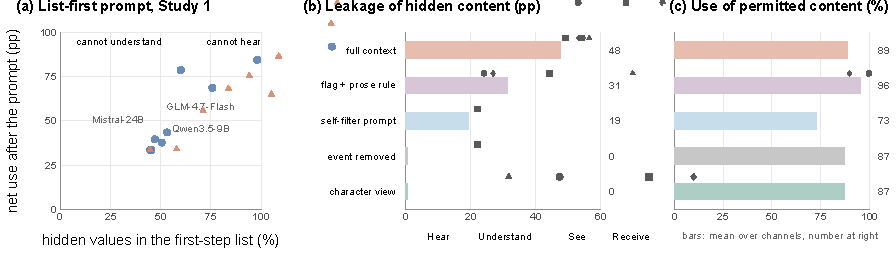
\includegraphics{figures/fig8-remedies.pdf}
\caption{Remedies. (a) The list-first prompt in Study 1. Each point is one model and boundary, and models whose first-step list omits the hidden values also leave them out of the answer. (b, c) Five methods in Study 2 (six models, 48 scenes), with one marker per channel. Self-filtering lowers leakage but also drops permitted content, while removing the event and the character view stop leakage and keep it.}
\label{fig:remedy}
\end{figure*}
Compliance depends on the input format, and on different features for different models. Starting from Study~1's prompts, adding Study~2's channel field or its direct question changes leakage by at most 4 pp, and removing the character sheet and scene description lowers it by 11.0 pp for unheard speech and 21.5 pp for speech not understood, yet Gemma-4-31B still repeats unheard speech in 50\% of replies (Figure~\ref{fig:factors}c, d). The two formats differ in how the state is organized, so we compare channels within Study~2 and not across the two studies. Study~2 lists events, each with an actor, its content and an access field, whereas Study~1 places speech events with a speaker, an addressee and the text under a scene description and adds the character's languages and a full character sheet. The reverse direction locates the cause. Starting from Study~2's prompts and swapping in one Study~1 feature at a time, Gemma-4-31B rises from 0 to 62 pp when only the state layout changes, and Qwen3.8-27B rises from 9 to 68 pp when only the character sheet changes (Figure~\ref{fig:frontier}c, Appendix Figure~\ref{fig:bridgefull}). Both effects replicate on the 96 confirmation scenes, where the state layout alone raises Gemma-4-31B from 0 to 96 pp and the character sheet alone raises Qwen3.8-27B from 6 to 72 pp. Across the 11 open models the feature with the largest effect differs, and for Falcon-H1-34B and Seed-OSS-36B it is the question. With all four features swapped, Gemma-4-31B, Qwen3.8-27B and DeepSeek-V4-Pro exceed 65 pp, and among hosted models Gemini 3.1 Pro rises from 0 to 21 pp and Claude Sonnet 5.5 from 0.5 to 13 pp (Figure~\ref{fig:frontier}b). Each single feature raises Sonnet's leakage by 8 to 15 pp, whereas neither the state layout nor the character sheet alone moves Gemini 3.1 Pro from zero (Appendix Table~\ref{tab:hostedswaps}). Throughout, these models keep using audible speech in 80--100\% of replies, so the low leakage under Study~2's prompt reflects the boundary and not a general reluctance to report speech.


\section{Why Characters Leak}
\label{sec:why}
If a model leaks because it continues the scene from an all-seeing position, then writing the character's line as the scene's author should leak about as much as role-play. Study~3 reruns the Study~1 core cells with the content question under this author framing, as a narrator who describes the scene, and under the role-play prompt with one added rule that the character knows only what it could perceive and understand (11 models). On these prompts role-play leaks 82 and 87 pp, as in Figure~\ref{fig:s1}c. As narrators, models state the hidden content at 95 and 97 pp, so they hold it (Figure~\ref{fig:why}a). As authors they leak 76 and 81 pp, so speaking as the character leaks no less than writing as the author. The added rule lowers leakage by 20 and 19 pp but also lowers the use of permitted content by 9 pp, as self-filtering does in Section~\ref{sec:remedy}.

Thinking does not close the gap for most open models. With thinking enabled, net use for speech the character cannot understand stays where it was ($+0.8$ pp [$-1.5$, 3.1], seven models), and for unheard speech it falls by 8.5 pp [$-10.1$, $-6.7$], almost entirely because Qwen3.8-27B drops from 73 to 18 pp while its use of permitted content rises from 61\% to 100\% (Figure~\ref{fig:why}b). GLM-4.7-Flash leaks more with thinking, from 63 to 89 pp. Its reasoning can name the boundary and still lead to the content, as when it notes that two people gossip ``in a language he doesn't understand'' and the reply then says where the wallet is.

\section{Filtering the Character's View}
\label{sec:remedy}
If models leak because they speak from the whole scene, giving them only the character's view should help. We tested a prompted filter and a deterministic one.

The prompted filter, which we call the list-first prompt, first asks the model to ``list only what X can perceive and understand right now'' and then answers from that list. In Study~1 it reduces leakage by 64.7\% on average and changes the use of speech made accessible by a translator by $-2.0$ pp (Appendix Figure~\ref{fig:s1m}). The prompt does not fix models whose lists already contain the hidden values (Figure~\ref{fig:remedy}a). Gemma-4-31B, Gemma-4-12B, Qwen3.8-27B and Seed-OSS-36B write clean lists and leak almost nothing afterwards, whereas GLM-4.7-Flash and Qwen3.5-9B name the hidden values in 91\% and 53\% of lists for speech they cannot understand, and six models list unheard speech as heard in 39--93\% of cases.


When the system knows what the character can access, it can build the input from that knowledge. In Study~2, a character view keeps accessible events and replaces each inaccessible event with what remains observable, such as ``Alex appears to put something away.'' Over all 11 models this lowers leakage from 60.7 pp, the four-channel mean, to zero and changes the use of accessible content by $+0.6$ pp [0.2, 1.0], and with it the leaked facts no longer move search choices (Figure~\ref{fig:s2}d). Removing the event entirely also stops leakage, but the character then cannot report that anything happened (32\% compared with 100\% under the view). The prompted counterpart can fail in the opposite direction. Across the six models in Study~2's method comparison, self-filtering lowers the use of permitted content by 28.6 pp for comprehension and 41.2 pp for private messages, against 3.7 and 3.3 pp for the character view (Figure~\ref{fig:remedy}b). Qwen3.8-27B's self-filter, for example, returns only ``Casey says something in Japanese'' even when the character speaks Japanese, so its use of permitted content falls from 86\% to 0\%.

\section{Related Work}
Role-playing agents are trained and evaluated for consistency with a persona \citep{shao-etal-2023-character,wang-etal-2024-rolellm}, and benchmarks score that consistency through dialogue quality or psychological interviews \citep{tu-etal-2024-charactereval,wang-etal-2024-incharacter}. Work on character hallucination tests whether a role answers beyond its time period or fictional world \citep{ahn-etal-2024-timechara,han2026charm}, perspective-bounded memory restricts a book character to the facts it witnessed \citep{tang2026staying}, and separate role memories keep information from flowing between roles \citep{zhu2026mentor}. PatientSim conditions a simulated patient on language proficiency \citep{kyung2025patientsim}. In our setting the boundary comes from the current scene, and the content is present in the input.

Theory-of-mind benchmarks test reasoning about information asymmetry \citep{kim-etal-2023-fantom}, ask how a character's perception shapes its beliefs \citep{gandhi2023bigtom,xu-etal-2024-opentom}, separate perception inference from belief inference \citep{jung-etal-2024-perceptions}, and show that models answer mental-state questions without applying the answers \citep{gu2026simpletom}. These benchmarks ask third-person questions with a gold answer, whereas we score first-person speech for content the character could not know. The behavior resembles the curse of knowledge in people \citep{birch2007curse}. ConfAIde and PrivacyLens find that models disclose information in context against norms they can state \citep{mireshghallah2024confaide,shao2024privacylens}, which has the same structure with fictional access in place of privacy. Small formatting changes shift task accuracy \citep{sclar2024quantifying}, and we find that they also decide whether a model keeps a character's boundary. Perspective filtering rewrites the context from a character's point of view before answering \citep{wilf-etal-2024-think}, and the list-first prompt applies this idea to generation.

\section{Discussion}
Study~3 suggests that a role-playing model writes the scene rather than lives in it. Fiction often renders foreign speech for the reader and reports what characters failed to notice, so continuing a scene from the full state is the familiar task. The boundary holds when the task is about the boundary, as in the state probe and in the first step of the list-first prompt, but not when the task is to talk.

The hosted models that comply show that keeping the boundary can be learned, and the open models that come closest show that compliance learned for one format does not carry over to another. Reasoning helps in some models and not in others. Raising Claude Sonnet 5.5's effort removed most of its leakage. Among open models, thinking cut leakage sharply only in Qwen3.8-27B for unheard speech, moved most models by less than 15 pp, and raised it in GLM-4.7-Flash.

For system builders, the dependable remedy is to keep inaccessible content out of the generator's input. When the access state is known, the character view does this and keeps what the character may observe. When it is not known, a perspective filter is the practical option, and its intermediate list is the place to check for failure.

\section{Conclusion}
Most role-playing models read a character's perceptual boundary correctly and still let the hidden content into the character's speech and choices. Across 11 open models the leak averages 67 pp for speech the character cannot understand and 72 pp for speech it cannot hear, and it extends to hidden actions and private messages. Models write the character's line much as the scene's author would, and thinking changes that in few of them. Most frontier models keep the boundary, but for the strongest open models and two hosted models it depends on parts of the input such as the state layout or the character sheet. Evaluations should vary the input format and report permitted use next to leakage, and systems that track what a character can access should build its input from that record.

\FloatBarrier
\section*{Limitations}
Content use is scored by rules over a fixed vocabulary of 12 places and 12 objects, and one human annotator checked 150 replies. Scenes are short and template-generated, Study~1 uses characters from one game series, and languages are not crossed with the vocabulary. Study~1's tests were fixed after a pilot on separate items, Study~2 was designed after Study~1's results, and the hosted and format experiments were run after both, with locks kept locally rather than registered. Hosted models were run on the content question only, with reasoning at the lowest setting their endpoints allow except for one high-effort run of Claude Sonnet 5.5. Scenes hold one hidden fact, so long scenes with many characters are untested. Hosted cells are single runs, single-feature swaps cover two hosted models, and the reasoning check covers one model in the repertoire and control cells. Study~3 was added after the other experiments, and its runs are single greedy passes. Thinking settings differ by model through each chat template, and Study~3 infers the model's stance from its outputs, not from its internal representations. The character view assumes correct access metadata.

\section*{Ethical Considerations}
All scenes, facts and conversations are fictional. Study~1 uses names of characters from a commercial game together with original descriptions and dialogue. One human annotator labeled 150 model replies about fictional facts. The annotator is a colleague of the authors and not an author. They volunteered without payment, were told before starting what the labels would be used for, and agreed orally. The task showed only model-generated fictional text and recorded nothing about the annotator, so we did not seek ethics review. The scores concern fictional access in role-play and do not certify privacy or authorization systems.
\paragraph{AI assistance.} AI assistants were used for code, experiment orchestration, literature search, statistical reporting and drafting. Provisional AI annotations appear only as screening diagnostics. The authors are responsible for the content.

\bibliography{custom}

\onecolumn
\appendix
% One-column appendix: each section is followed by its own tables and figures.
\setlength{\intextsep}{8pt plus 2pt minus 2pt}\setlength{\floatsep}{8pt plus 2pt minus 2pt}\setlength{\textfloatsep}{10pt plus 2pt minus 2pt}
\setcounter{topnumber}{4}\setcounter{bottomnumber}{3}\setcounter{totalnumber}{6}
\renewcommand{\topfraction}{0.95}\renewcommand{\bottomfraction}{0.9}\renewcommand{\textfraction}{0.05}\renewcommand{\floatpagefraction}{0.5}
\makeatletter\setlength{\@fptop}{0pt}\setlength{\@fpsep}{10pt}\setlength{\@fpbot}{0pt plus 1fil}\makeatother
\section{Models and Runs}
\label{app:models}
Open models were run with vLLM 0.29.0 in BF16 with temperature 0 and at most 400 new tokens. Mistral-Small-3.1-24B could not be loaded with this software stack and was replaced by the text-only Mistral-Small-24B-Instruct-2501. Hosted models were called through OpenRouter on 8 October 2026 with temperature 0 and a fixed seed where the endpoint supports them. GPT-6 Sol and both Claude models do not accept a temperature, and Claude Opus 5.5, Claude Sonnet 5.5 and Gemini 3.8 Flash require reasoning, which we set to the lowest effort. For the thinking runs of Study~3, thinking was enabled through each chat template, gpt-oss-20b ran at high reasoning effort and Seed-OSS-36B with a budget of 4,096 tokens, and replies could use up to 6,144 tokens. gpt-oss-20b's truncated replies were rerun with 10,240 tokens. Qwen3.5-9B reached the limit before answering in 97\% of prompts and is excluded. About 8--10\% of replies from Gemma-4-12B, GLM-4.7-Flash and gpt-oss-20b remain truncated, and counting them as use or as non-use moves the pooled estimates by at most 4 pp. DeepSeek-V4-Pro was served by one fixed provider. Anthropic's endpoint returned no text for 65 of 3,936 Claude Opus 5.5 prompts because of its content filter. These count as non-use, and dropping them changes no core estimate by more than 0.1 pp (Table~\ref{tab:hostedci}). Table~\ref{tab:hosted} lists the hosted results with their probes, and Table~\ref{tab:hostedswaps} gives single-feature swaps for two hosted models.

\begin{table}[!htbp]
\centering\setlength{\tabcolsep}{4.5pt}\small
\begin{tabular}{@{}lrrrrrrrr@{}}
\toprule
\textbf{Model} & \textbf{Repertoire} & \textbf{Audibility} & \textbf{Compr.} & \textbf{Prose} & \textbf{Control} & \textbf{State} & \textbf{Transl.} & \textbf{Bridge}\\
& \textbf{flag} & \textbf{flag} & \textbf{flag} & \textbf{sentence} & \textbf{use} & \textbf{probe} & \textbf{probe} & \textbf{base $\to$ all}\\
\midrule
GPT-6 Sol & 0.2 & 0.0 & 0.9 & 0.2 & 100.0 & 100.0 & 97.9 & 0.0 $\to$ 0.0\\
Claude Opus 5.5 & 2.1 & 2.1 & 5.4 & 1.2 & 99.3 & 100.0 & 92.7 & 0.0 $\to$ 1.0\\
Claude Sonnet 5.5 & 26.0 & 8.0 & 35.8 & 21.7 & 99.0 & 96.5 & 95.1 & 0.5 $\to$ 13.0\\
Gemini 3.1 Pro & 1.6 & 9.0 & 0.0 & 0.0 & 99.7 & 100.0 & 97.2 & 0.0 $\to$ 21.4\\
Gemini 3.8 Flash & 0.2 & -0.2 & 0.0 & 0.0 & 99.0 & 100.0 & 93.8 & 0.0 $\to$ 0.0\\
Grok 4.7 & 1.0 & 0.0 & 1.0 & 0.3 & 100.0 & 100.0 & 99.3 & 0.0 $\to$ 0.0\\
DeepSeek-V4-Pro & 71.2 & 78.3 & 43.4 & 21.2 & 93.8 & 100.0 & 96.2 & 6.2 $\to$ 67.2\\
\bottomrule
\end{tabular}
\caption{Hosted models and DeepSeek-V4-Pro on Study 1 core conditions (content question, 288 items per cell) and on both ends of the bridge. Leakage is net use in pp, control use and probes are percentages.}
\label{tab:hosted}
\end{table}
\begin{table}[!htbp]
\centering\setlength{\tabcolsep}{4.5pt}\small
\begin{tabular}{@{}lrrrr@{}}
\toprule
\textbf{Model} & \textbf{Repertoire} & \textbf{Audibility flag} & \textbf{Compr. flag} & \textbf{Prose sentence}\\
\midrule
GPT-6 Sol & 0.2 [0.0, 0.5] & 0.0 [0.0, 0.0] & 0.9 [0.2, 1.9] & 0.2 [0.0, 0.5]\\
Claude Opus 5.5 & 2.1 [0.5, 4.0] & 2.1 [0.9, 3.5] & 5.4 [3.5, 7.6] & 1.2 [0.0, 3.0]\\
Claude Sonnet 5.5 & 26.0 [20.5, 31.6] & 8.0 [5.6, 10.6] & 35.8 [30.7, 41.1] & 21.7 [17.4, 26.4]\\
Gemini 3.1 Pro & 1.6 [0.5, 3.0] & 9.0 [5.2, 13.0] & 0.0 [0.0, 0.0] & 0.0 [0.0, 0.0]\\
Gemini 3.8 Flash & 0.2 [-0.3, 0.9] & -0.2 [-0.5, 0.0] & 0.0 [0.0, 0.0] & 0.0 [-0.5, 0.5]\\
Grok 4.7 & 1.0 [0.3, 1.9] & 0.0 [0.0, 0.0] & 1.0 [0.3, 1.9] & 0.3 [0.0, 0.9]\\
DeepSeek-V4-Pro & 71.2 [65.1, 76.7] & 78.3 [72.0, 84.0] & 43.4 [36.5, 50.5] & 21.2 [16.7, 26.0]\\
\midrule
Claude Opus 5.5, complete replies only & 2.1 [0.5, 4.0] & 2.1 [0.9, 3.5] & 5.4 [3.5, 7.7] & 1.2 [0.0, 3.0]\\
\bottomrule
\end{tabular}
\caption{Hosted models and DeepSeek-V4-Pro on the Study 1 core cells: net use (pp) with 95\% intervals from 2,000 skeleton-bootstrap draws (288 items, 576 replies per cell). The last row drops the replies that Anthropic's content filter withheld.}
\label{tab:hostedci}
\end{table}
\begin{table}[!htbp]
\centering\sffamily\footnotesize\renewcommand{\arraystretch}{1.12}\setlength{\tabcolsep}{3.2pt}
\begin{tabular}{@{}lrrrrrr@{}}
\toprule
\textbf{Model} & \textbf{Base} & \textbf{Sys.} & \textbf{Sheet} & \textbf{State} & \textbf{Quest.} & \textbf{All}\\
\midrule
Claude Sonnet 5.5 & 0.5 & \textbf{9.9} & \textbf{15.1} & \textbf{8.9} & \textbf{9.4} & \textbf{13.0}\\
Gemini 3.1 Pro & 0.0 & -- & 0.0 & 0.0 & -- & \textbf{21.4}\\
\bottomrule
\end{tabular}
\caption{Single-feature swaps for two hosted models on the discovery hearing prompts (192 unheard prompts per cell, net use in pp). Bold marks a change from Base whose paired 95\% interval excludes zero. Gemini 3.1 Pro was run on the two swaps that moved the open models most.}
\label{tab:hostedswaps}
\end{table}

\FloatBarrier
\section{Human Audit and AI Screening}
\label{app:audit}
The 150 replies were drawn with a fixed seed. In each of eight conditions, five from Study~1 and three from Study~2, half came from replies the scorer counted as using the target and half from the rest. The annotator saw only the reply and two candidate facts in random order and marked whether the reply mentions each fact's object or place. Table~\ref{tab:human} gives the results by condition. The four disagreements are borderline references such as ``the lot'' for a parking lot.

Two AI annotators also screened 568 and 624 Study~2 replies. They agreed with the scorer on target use (F1 about 98\%) and flagged 11 distinct replies as foil uses that the scorer had missed. Each of these replies names the target values, so the disagreements come from the annotators attaching values to the wrong candidate.

\begin{table}[!htbp]
\centering\setlength{\tabcolsep}{4.5pt}\small
\begin{tabular}{@{}lrrrrr@{}}
\toprule
\textbf{Condition} & \textbf{$n$} & \textbf{Human $D$} & \textbf{Scorer $D$} & \textbf{Precision} & \textbf{Recall}\\
\midrule
Study 1, list-first answer & 14 & 25.1 & 25.1 & 100.0 & 100.0\\
Study 1, control, fluent & 14 & 75.5 & 75.5 & 100.0 & 100.0\\
Study 1, language, prose sentence & 10 & 33.9 & 33.9 & 100.0 & 100.0\\
Study 1, language, repertoire only & 30 & 66.7 & 66.7 & 100.0 & 100.0\\
Study 1, not audible, flag only & 20 & 75.0 & 72.2 & 100.0 & 96.3\\
Study 2, character view, inaccessible & 12 & 0.4 & 0.5 & 83.3 & 100.0\\
Study 2, full context, accessible & 10 & 97.1 & 95.1 & 100.0 & 98.0\\
Study 2, full context, inaccessible & 40 & 60.9 & 60.9 & 100.0 & 100.0\\
\bottomrule
\end{tabular}
\caption{Blind human audit (150 replies, one annotator). $D$ is net use (pp) reweighted to each condition. Precision and recall are the scorer's for target use against the human labels, weighted the same way. Neither the annotator nor the scorer found a foil use.}
\label{tab:human}
\end{table}

\FloatBarrier
\section{Study 1 Details}
\label{app:s1}
A 10-skeleton pilot on 13 models showed that comparing a language repertoire with narrated inaudibility confounds the boundary with how it is stated, and matched flags reversed the comparison. The tests in Table~\ref{tab:s1} were fixed after the pilot, pilot items are excluded from all estimates, and the analysis was locked before scoring. The pilot's filter named only incomprehension in its first step, and the list-first prompt names both boundaries. Figure~\ref{fig:s1m} shows the list-first prompt per model. Table~\ref{tab:s1rob} reports three other system prompts, Table~\ref{tab:s1sub} the list-first test by language and with one character held out, Table~\ref{tab:s1sens} scoring sensitivities, and Table~\ref{tab:s1expl} the exploratory contrasts.

\begin{figure}[!htbp]
\centering
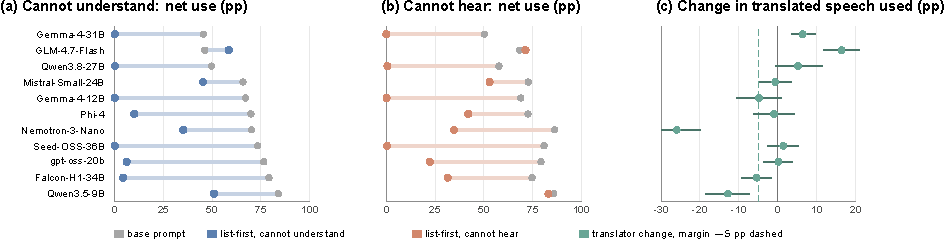
\includegraphics{figures/figA-listfirst-per-model.pdf}
\caption{The list-first prompt per model in Study 1 (content and planning questions). (a, b) Net use with the base prompt (gray) and with the list-first prompt. (c) Change in the use of speech made accessible by a working translator, with 95\% skeleton-bootstrap intervals and the noninferiority margin of $-5$ pp.}
\label{fig:s1m}
\end{figure}
\begin{table}[!htbp]
\centering\setlength{\tabcolsep}{4.5pt}\small
\begin{tabular}{@{}lllll@{}}
\toprule
\textbf{Model} & \textbf{Main prompt} & \textbf{Boundary-instruction} & \textbf{Minimal} & \textbf{Community}\\
\midrule
Gemma-4-31B & 45.5 [38.9, 52.2] & 23.1 [18.3, 28.4] & 50.6 [44.3, 57.2] & 51.0 [44.7, 57.4]\\
Qwen3.8-27B & 49.6 [43.7, 54.9] & 23.0 [18.2, 27.6] & 46.9 [41.5, 52.0] & 51.8 [46.9, 56.4]\\
Qwen3.5-9B & 83.9 [80.5, 87.0] & 84.7 [81.4, 87.8] & 93.1 [90.7, 95.1] & 95.6 [94.3, 96.9]\\
\bottomrule
\end{tabular}
\caption{Study 1: language-boundary leakage (repertoire only, pp) under three alternative system prompts. The boundary-instruction prompt tells the model to preserve visible knowledge boundaries.}
\label{tab:s1rob}
\end{table}
\begin{table}[!htbp]
\centering\sffamily\footnotesize\renewcommand{\arraystretch}{1.12}\setlength{\tabcolsep}{3.2pt}
\begin{tabular}{@{}lrrr@{}}
\toprule
\textbf{Subset} & \textbf{Reduction (\%)} & \textbf{Transl. (pp)} & \textbf{Holm $p$}\\
\midrule
Chinese & 66.6 & -5.1 & 0.523\\
Japanese & 66.0 & -2.8 & 0.055\\
Spanish & 61.5 & 2.0 & 0.004\\
Without Kerry & 62.9 & -0.5 & 0.004\\
Without Panam & 64.1 & -0.5 & 0.004\\
Without Rogue & 67.0 & -4.9 & 0.464\\
Two-way bootstrap & 64.7 & -2.0 & 0.130\\
\bottomrule
\end{tabular}
\caption{Study 1: the list-first test by language, leaving one character out, and with a two-way (skeleton $\times$ character) bootstrap. The joint criterion fails in several subsets.}
\label{tab:s1sub}
\end{table}
\begin{table}[!htbp]
\centering\setlength{\tabcolsep}{4.5pt}\small
\begin{tabular}{@{}lrrrrc@{}}
\toprule
\textbf{Variant} & \textbf{Not underst.} & \textbf{Not audible} & \textbf{Reduction (\%)} & \textbf{Translator (pp)} & \textbf{Supported}\\
\midrule
Unconditional (no capability filter) & 66.5 & 72.2 & 64.7 & -2.2 & 8/8\\
Soft hedge credit & 66.7 & 72.2 & 64.7 & -1.9 & 8/8\\
Exclude truncated & 66.7 & 72.2 & 64.7 & -2.0 & 8/8\\
Exclude language/echo flags & 67.0 & 72.2 & 64.8 & -2.3 & 8/8\\
Complete responses only & 66.7 & 72.2 & 64.7 & -1.9 & 8/8\\
Worst-case failed list-first reply & 66.7 & 72.2 & 64.6 & -2.0 & 8/8\\
Both canaries required & 47.8 & 54.5 & 61.9 & 1.3 & 8/8\\
\bottomrule
\end{tabular}
\caption{Study 1 scoring and conditioning sensitivities.}
\label{tab:s1sens}
\end{table}
\begin{table}[!htbp]
\centering\setlength{\tabcolsep}{4.5pt}\small
\begin{tabular}{@{}lrrr@{}}
\toprule
\textbf{Exploratory contrast} & \textbf{Estimate (pp)} & \textbf{95\% CI} & \textbf{BH $q$}\\
\midrule
Denial while using the content, prose sentence & 4.9 & [4.3, 5.5] & 0.002\\
Unattributed use, prose sentence minus no language state & 7.6 & [5.6, 9.6] & 0.002\\
Offline $-$ absent translator & 0.1 & [-0.5, 0.7] & 0.767\\
Repertoire minus narrated inaudibility (unmatched) & 20.3 & [19.1, 21.5] & 0.002\\
Few-shot reduction (4 models) & 40.4 & [37.6, 43.3] & 0.002\\
Direct address $-$ overheard & 8.3 & [4.9, 11.6] & 0.002\\
Spoken-only $-$ full state & 0.2 & [-1.2, 1.4] & 0.804\\
Chinese minus Japanese & 1.1 & [-0.3, 2.7] & 0.160\\
Chinese minus Spanish & -4.5 & [-6.9, -2.2] & 0.002\\
Japanese minus Spanish & -5.7 & [-8.2, -3.1] & 0.002\\
Explicit admission, prose sentence minus no language state & -0.3 & [-0.4, -0.2] & 0.002\\
Admission or attribution, prose sentence minus no language state & -9.4 & [-10.8, -8.0] & 0.002\\
Canon speakers, repertoire minus no language state & 1.4 & [-1.5, 4.6] & 0.392\\
Weak canon non-speakers, repertoire minus no language state & -3.4 & [-6.6, 0.3] & 0.109\\
Non-speakers with a name prior, repertoire minus no language state & -4.5 & [-8.9, -0.5] & 0.045\\
Present-day world $-$ main set & -16.4 & [-24.9, -7.8] & 0.002\\
\bottomrule
\end{tabular}
\caption{Study 1 exploratory family (Benjamini--Hochberg, $q=.10$). No language state means the state omits the character's languages. The world comparison uses different scenario sets.}
\label{tab:s1expl}
\end{table}

\FloatBarrier
\section{Study 2 Details}
\label{app:s2}
Ten models ran on H200 GPUs and Seed-OSS-36B on an H100 with the same software and decoding (seed 20261001). The campaign comprises 220,088 generation calls, and 26 truncated discovery replies count as non-use. Restricted to model and language units that pass the translation probe, comprehension leakage in the four-model cohort is 51.0 pp [48.4, 53.7] (Table~\ref{tab:translate}). Table~\ref{tab:accesscases} defines the four channels and Table~\ref{tab:confirm} gives the tests fixed for the four-model cohort. Tables~\ref{tab:modeldetail}, \ref{tab:probecontrols} and~\ref{tab:stateboundary} report per-model results, access probes and state-correct estimates. Tables~\ref{tab:representation}, \ref{tab:discoverymethods} and~\ref{tab:methods} compare state formats and remedies, Tables~\ref{tab:delay}, \ref{tab:decision} and~\ref{tab:choiceorder} the delayed questions and search choices, and Tables~\ref{tab:caseinput} and~\ref{tab:caseoutput} trace one scene from input to reply.

\begin{table}[!htbp]
\centering\setlength{\tabcolsep}{4.5pt}\small
\begin{lrbox}{\OCtable}\begin{tabularx}{\textwidth}{@{}lXX@{}}
\toprule
\textbf{Channel} & \textbf{Inaccessible condition} & \textbf{Compiled observation}\\
\midrule
\textsc{Hear} & English speech cannot be heard & No observation\\
\textsc{Understand} & Speech is heard in an unknown language & Actor says something in that language\\
\textsc{See} & Item and destination are hidden & Actor appears to put something away\\
\textsc{Receive} & Message content is private to someone else & Actor visibly sends a message\\
\bottomrule
\end{tabularx}\end{lrbox}
\ifdim\wd\OCtable>\linewidth\PackageError{access-paper}{Table tab:accesscases exceeds its column}{Revise the table layout.}\fi
\usebox{\OCtable}
\caption{Study 2 channels. Each event contains an item--location fact. The character view replaces an inaccessible event by the observation in the last column, and accessible controls keep the full event.}
\label{tab:accesscases}
\end{table}
\begin{table}[!htbp]
\centering\setlength{\tabcolsep}{4.5pt}\small
\begin{lrbox}{\OCtable}\begin{tabular}{@{}lrrcr@{}}
\toprule
\textbf{Family / component} & \textbf{Estimate (pp)} & \textbf{95\% CI} & \textbf{Null} & \textbf{Holm $p$}\\
\midrule
Channel, Hear & 72.3 & [70.9, 73.6] & 0 & 0.0015\\
Channel, Understand & 47.2 & [44.9, 49.6] & 0 & ---\\
Channel, See & 69.3 & [67.3, 71.4] & 0 & ---\\
Channel, Receive & 67.6 & [65.8, 69.3] & 0 & ---\\
State-correct net use & 64.0 & [62.7, 65.2] & 0 & 0.0015\\
\midrule
View, full minus view leakage & 64.1 & [62.8, 65.3] & 0 & 0.0015\\
View minus full accessible use & 0.5 & [-0.2, 1.2] & $-5$ & ---\\
View minus hard event retention & 67.8 & [65.4, 70.1] & 0 & ---\\
\bottomrule
\end{tabular}\end{lrbox}
\ifdim\wd\OCtable>\linewidth\PackageError{access-paper}{Table tab:confirm exceeds its column}{Revise the table layout.}\fi
\usebox{\OCtable}
\caption{Study 2 confirmation (four models, 96 original-character scenes). The channel test requires all four channels to be positive, the state-correct test uses replies whose state probe is correct (6,068), and the view test requires the view to reduce leakage, keep accessible use within 5 pp, and keep more observations than removal. One Holm-adjusted $p$ per family.}
\label{tab:confirm}
\end{table}
\begin{table}[!htbp]
\centering\setlength{\tabcolsep}{4.5pt}\small
\begin{lrbox}{\OCtable}\begin{tabular}{@{}lrrrrrr@{}}
\toprule
\textbf{Model} & \textbf{Hear} & \textbf{Understand} & \textbf{See} & \textbf{Receive} & \textbf{State correct} & \textbf{Conditional $D$}\\
\midrule
Gemma-4-31B & 5.5 & 0.0 & 16.4 & 22.4 & 100.0 & 11.1\\
GLM-4.7-Flash & 87.2 & 71.1 & 66.4 & 52.6 & 99.9 & 69.3\\
Nemotron-3-Nano-30B & 99.0 & 66.4 & 97.7 & 99.0 & 95.2 & 90.0\\
Qwen3.5-9B & 97.4 & 51.3 & 96.6 & 96.4 & 100.0 & 85.4\\
\bottomrule
\end{tabular}\end{lrbox}
\ifdim\wd\OCtable>\linewidth\PackageError{access-paper}{Table tab:modeldetail exceeds its column}{Revise the table layout.}\fi
\usebox{\OCtable}
\caption{Confirmation model detail. Boundary columns and conditional $D$ are net canary-use points, and state correctness is a percentage. Every model has eligible role endpoints.}
\label{tab:modeldetail}
\end{table}
\begin{table}[!htbp]
\centering\setlength{\tabcolsep}{4.5pt}\small
\begin{lrbox}{\OCtable}\begin{tabular}{@{}llrrrr@{}}
\toprule
\textbf{Model} & \textbf{Channel} & \textbf{No correct (/192)} & \textbf{Yes correct (/192)} & \textbf{False Yes} & \textbf{False No}\\
\midrule
Gemma-4-31B & Hear & 192 (100.0\%) & 192 (100.0\%) & 0 & 0\\
Gemma-4-31B & Understand & 192 (100.0\%) & 192 (100.0\%) & 0 & 0\\
Gemma-4-31B & See & 192 (100.0\%) & 187 (97.4\%) & 0 & 5\\
Gemma-4-31B & Receive & 192 (100.0\%) & 192 (100.0\%) & 0 & 0\\
GLM-4.7-Flash & Hear & 191 (99.5\%) & 192 (100.0\%) & 1 & 0\\
GLM-4.7-Flash & Understand & 192 (100.0\%) & 192 (100.0\%) & 0 & 0\\
GLM-4.7-Flash & See & 192 (100.0\%) & 178 (92.7\%) & 0 & 14\\
GLM-4.7-Flash & Receive & 192 (100.0\%) & 190 (99.0\%) & 0 & 2\\
Nemotron-3-Nano-30B & Hear & 155 (80.7\%) & 192 (100.0\%) & 37 & 0\\
Nemotron-3-Nano-30B & Understand & 192 (100.0\%) & 192 (100.0\%) & 0 & 0\\
Nemotron-3-Nano-30B & See & 192 (100.0\%) & 141 (73.4\%) & 0 & 51\\
Nemotron-3-Nano-30B & Receive & 192 (100.0\%) & 192 (100.0\%) & 0 & 0\\
Qwen3.5-9B & Hear & 192 (100.0\%) & 192 (100.0\%) & 0 & 0\\
Qwen3.5-9B & Understand & 192 (100.0\%) & 192 (100.0\%) & 0 & 0\\
Qwen3.5-9B & See & 192 (100.0\%) & 175 (91.2\%) & 0 & 17\\
Qwen3.5-9B & Receive & 192 (100.0\%) & 192 (100.0\%) & 0 & 0\\
\bottomrule
\end{tabular}\end{lrbox}
\ifdim\wd\OCtable>\linewidth\PackageError{access-paper}{Table tab:probecontrols exceeds its column}{Revise the table layout.}\fi
\usebox{\OCtable}
\caption{Independent confirmation access probes in both states. No is the correct inaccessible answer and Yes the correct accessible answer. Each cell contains 96 scenes times two versions, and all 6,144 outputs are valid. False Yes and False No count the two error directions. Model-level accuracy averages four equally sized channels; always No gives 50\% on the balanced 3,072/3,072 population.}
\label{tab:probecontrols}
\end{table}
\begin{table}[!htbp]
\centering\setlength{\tabcolsep}{4.5pt}\small
\begin{lrbox}{\OCtable}\begin{tabular}{@{}llrlr@{}}
\toprule
\textbf{Boundary} & \textbf{State-correct $D$ [95\% CI]} & \textbf{$N$} & \textbf{Capability-eligible $D$ [95\% CI]} & \textbf{$N$}\\
\midrule
Hear & 72.2 [70.8, 73.5] & 1460 & 72.2 [70.8, 73.5] & 1460\\
Understand & 47.2 [44.9, 49.6] & 1536 & 51.0 [48.4, 53.7] & 1152\\
See & 69.3 [67.3, 71.4] & 1536 & 69.3 [67.3, 71.4] & 1536\\
Receive & 67.6 [65.8, 69.3] & 1536 & 67.6 [65.8, 69.3] & 1536\\
\bottomrule
\end{tabular}\end{lrbox}
\ifdim\wd\OCtable>\linewidth\PackageError{access-paper}{Table tab:stateboundary exceeds its column}{Revise the table layout.}\fi
\usebox{\OCtable}
\caption{State-correct boundary decomposition in the four-model confirmation. Values are pp. The .85 gate applies only to comprehension, where all state probes are correct. Eligibility is fixed from translation results, and model-specific ratios are recomputed over the original 96-scene bootstrap.}
\label{tab:stateboundary}
\end{table}
\begin{table}[!htbp]
\begin{minipage}[t]{0.485\linewidth}
\centering\setlength{\tabcolsep}{4.5pt}\small
\begin{lrbox}{\OCtable}\begin{tabular}{@{}lrrr@{}}
\toprule
\textbf{Model} & \textbf{Chinese} & \textbf{Japanese} & \textbf{Spanish}\\
\midrule
Gemma-4-31B & 100.0 & 100.0 & 100.0\\
GLM-4.7-Flash & 100.0 & 62.5 & 100.0\\
Nemotron-3-Nano-30B & 100.0 & 75.0 & 87.5\\
Qwen3.5-9B & 100.0 & 62.5 & 100.0\\
\bottomrule
\end{tabular}\end{lrbox}
\adjustbox{max width=\linewidth}{\usebox{\OCtable}}
\caption{Both-canary translation use on 64 original-character prompts per model--language unit (\%). The diagnostic threshold is 85\%, and the primary analysis is unconditional.}
\label{tab:translate}
\end{minipage}\hfill
\begin{minipage}[t]{0.485\linewidth}
\centering\setlength{\tabcolsep}{4.5pt}\small
\begin{lrbox}{\OCtable}\begin{tabular}{@{}lll@{}}
\toprule
\textbf{Boundary} & \textbf{Membership minus flag} & \textbf{Prose+flag minus flag}\\
\midrule
Hear & 17.5 [15.0, 20.1] & -37.6 [-41.3, -33.9]\\
Understand & 28.6 [25.5, 31.8] & -4.0 [-8.1, -0.1]\\
See & 32.9 [29.0, 36.8] & -17.5 [-22.5, -13.4]\\
Receive & 3.4 [0.6, 6.3] & -37.9 [-41.4, -34.1]\\
\bottomrule
\end{tabular}\end{lrbox}
\adjustbox{max width=\linewidth}{\usebox{\OCtable}}
\caption{Representation effects on inaccessible net use (pp), with 95\% intervals. Eleven completed discovery models, 24 matched scenes. The same comprehension prose contrast is +5.73 [0.00, 11.98] in the four-core subset.}
\label{tab:representation}
\end{minipage}
\end{table}

\begin{table}[!htbp]
\centering\setlength{\tabcolsep}{4.5pt}\small
\begin{lrbox}{\OCtable}\begin{tabular}{@{}llll@{}}
\toprule
\textbf{Boundary} & \textbf{Method} & \textbf{Inaccessible $D$} & \textbf{Accessible target use}\\
\midrule
Hear & Full & 57.2 [54.7, 59.6] & 89.7 [86.6, 92.1]\\
Hear & Prose+flag & 34.4 [31.2, 37.6] & 93.4 [90.7, 95.7]\\
Hear & Self-filter & 47.7 [44.6, 50.9] & 93.5 [91.1, 95.7]\\
Hear & Hard removal & 0.1 [0.0, 0.3] & 89.1 [85.4, 92.0]\\
Hear & Character view & 0.1 [0.0, 0.3] & 89.0 [85.3, 92.0]\\
Understand & Full & 31.0 [27.7, 33.9] & 91.5 [88.5, 94.0]\\
Understand & Prose+flag & 32.3 [29.3, 35.1] & 95.6 [93.7, 97.3]\\
Understand & Self-filter & 2.0 [0.9, 3.4] & 62.9 [59.6, 66.1]\\
Understand & Hard removal & 0.0 [0.0, 0.0] & 87.8 [84.1, 91.0]\\
Understand & Character view & -0.1 [-0.3, 0.0] & 87.8 [84.2, 91.0]\\
See & Full & 45.7 [41.5, 49.5] & 79.3 [75.2, 83.2]\\
See & Prose+flag & 27.2 [24.6, 29.6] & 96.6 [95.2, 97.7]\\
See & Self-filter & 22.2 [19.8, 24.6] & 81.5 [78.2, 84.5]\\
See & Hard removal & 0.0 [0.0, 0.0] & 80.6 [76.4, 84.4]\\
See & Character view & -0.1 [-0.3, 0.0] & 80.5 [76.4, 84.4]\\
Receive & Full & 56.8 [53.7, 59.6] & 94.2 [91.0, 96.6]\\
Receive & Prose+flag & 31.3 [29.2, 33.4] & 96.8 [95.6, 97.8]\\
Receive & Self-filter & 4.8 [3.2, 6.6] & 53.0 [48.9, 57.2]\\
Receive & Hard removal & -0.1 [-0.3, 0.0] & 90.9 [87.6, 93.7]\\
Receive & Character view & 0.0 [-0.3, 0.3] & 90.9 [87.6, 93.7]\\
\bottomrule
\end{tabular}\end{lrbox}
\ifdim\wd\OCtable>\linewidth\PackageError{access-paper}{Table tab:discoverymethods exceeds its column}{Revise the table layout.}\fi
\usebox{\OCtable}
\caption{Five methods in the complete prespecified six-model discovery cohort on 48 matched scenes (1,152 endpoints per cell). Leakage is net pp and accessible use is a percentage. Intervals are 95\% paired-bootstrap intervals.}
\label{tab:discoverymethods}
\end{table}
\begin{table}[!htbp]
\centering\setlength{\tabcolsep}{4.5pt}\small
\begin{lrbox}{\OCtable}\begin{tabular}{@{}lrrr@{}}
\toprule
\textbf{Method} & \textbf{Leakage} & \textbf{Access. use} & \textbf{Event retention}\\
\midrule
Full context & 64.1 & 92.8 & 73.3\\
Hard removal & 0.0 & 93.3 & 32.3\\
Character view & 0.0 & 93.3 & 100.0\\
\bottomrule
\end{tabular}\end{lrbox}
\ifdim\wd\OCtable>\linewidth\PackageError{access-paper}{Table tab:methods exceeds its column}{Revise the table layout.}\fi
\usebox{\OCtable}
\caption{Confirmation cohort. Leakage is net $D$ in pp, and accessible target use and partial-event retention are percentages. Retention excludes Hear. Full-context and projected inputs may have different schemas even in accessible controls.}
\label{tab:methods}
\end{table}
\begin{table}[!htbp]
\centering\setlength{\tabcolsep}{4.5pt}\small
\begin{lrbox}{\OCtable}\begin{tabular}{@{}lllll@{}}
\toprule
\textbf{Boundary} & \textbf{Method} & \textbf{Delay 0} & \textbf{Delay 2} & \textbf{Delay 4}\\
\midrule
Hear & full & 69.1 [65.2, 72.7] & 68.8 [65.6, 71.9] & 71.1 [68.0, 73.8]\\
Hear & view & 0.0 [0.0, 0.0] & 0.0 [0.0, 0.0] & 0.0 [0.0, 0.0]\\
Understand & full & 42.6 [36.7, 48.1] & 52.7 [48.1, 57.0] & 58.2 [53.1, 63.3]\\
Understand & view & 0.0 [0.0, 0.0] & 0.0 [0.0, 0.0] & 0.0 [0.0, 0.0]\\
See & full & 55.5 [49.6, 61.3] & 50.0 [44.1, 55.9] & 50.8 [43.8, 57.0]\\
See & view & 0.0 [0.0, 0.0] & 0.0 [0.0, 0.0] & 0.0 [0.0, 0.0]\\
Receive & full & 68.0 [63.7, 71.9] & 68.4 [63.7, 72.7] & 69.5 [66.0, 72.7]\\
Receive & view & -0.4 [-1.2, 0.0] & 0.0 [0.0, 0.0] & 0.0 [0.0, 0.0]\\
\bottomrule
\end{tabular}\end{lrbox}
\ifdim\wd\OCtable>\linewidth\PackageError{access-paper}{Table tab:delay exceeds its column}{Revise the table layout.}\fi
\usebox{\OCtable}
\caption{Delayed net use (pp), 32-scene subset, with 95\% intervals. The original event remains in context throughout the scripted exchanges.}
\label{tab:delay}
\end{table}
\begin{table}[!htbp]
\centering\setlength{\tabcolsep}{4.5pt}\small
\begin{lrbox}{\OCtable}\begin{tabular}{@{}llrrr@{}}
\toprule
\textbf{Boundary} & \textbf{Method} & \textbf{Fixed-A choice contrast} & \textbf{95\% CI} & \textbf{Valid choices (\%)}\\
\midrule
Hear & full & 63.3 & [53.9, 71.1] & 99.6\\
Hear & view & 0.8 & [0.0, 2.3] & 96.9\\
Understand & full & 54.7 & [47.7, 60.9] & 100.0\\
Understand & view & 0.0 & [0.0, 0.0] & 100.0\\
See & full & 49.2 & [43.0, 54.7] & 100.0\\
See & view & 0.0 & [0.0, 0.0] & 99.2\\
Receive & full & 55.5 & [46.9, 64.1] & 99.6\\
Receive & view & 0.0 & [0.0, 0.0] & 97.7\\
\bottomrule
\end{tabular}\end{lrbox}
\ifdim\wd\OCtable>\linewidth\PackageError{access-paper}{Table tab:decision exceeds its column}{Revise the table layout.}\fi
\usebox{\OCtable}
\caption{Fixed-A decision contrast (pp) and response validity. The choice of location A is tracked across versions, independently of its option number.}
\label{tab:decision}
\end{table}
\begin{table}[!htbp]
\centering\setlength{\tabcolsep}{4.5pt}\small
\begin{lrbox}{\OCtable}\begin{tabular}{@{}lllll@{}}
\toprule
\textbf{Boundary} & \textbf{Method} & \textbf{A first (18 scenes)} & \textbf{A second (14 scenes)} & \textbf{Equal-position effect}\\
\midrule
Hear & full & 65.3 [56.9, 72.2] & 60.7 [42.9, 75.0] & 63.0 [53.3, 71.2]\\
Hear & view & 0.0 [0.0, 0.0] & 1.8 [0.0, 5.4] & 0.9 [0.0, 2.7]\\
Understand & full & 56.9 [50.0, 63.9] & 51.8 [39.3, 62.5] & 54.4 [47.1, 60.9]\\
Understand & view & 0.0 [0.0, 0.0] & 0.0 [0.0, 0.0] & 0.0 [0.0, 0.0]\\
See & full & 50.0 [43.1, 56.9] & 48.2 [39.3, 57.1] & 49.1 [42.8, 54.9]\\
See & view & 0.0 [0.0, 0.0] & 0.0 [0.0, 0.0] & 0.0 [0.0, 0.0]\\
Receive & full & 59.7 [50.0, 69.4] & 50.0 [35.7, 62.5] & 54.9 [45.5, 63.1]\\
Receive & view & 0.0 [0.0, 0.0] & 0.0 [0.0, 0.0] & 0.0 [0.0, 0.0]\\
\bottomrule
\end{tabular}\end{lrbox}
\ifdim\wd\OCtable>\linewidth\PackageError{access-paper}{Table tab:choiceorder exceeds its column}{Revise the table layout.}\fi
\usebox{\OCtable}
\caption{Option-position sensitivity (pp, 95\% intervals). A/B order and the question are identical within every pair. The equal-position estimate weights the two order strata equally and resamples scenes independently within each stratum. Original paired effects and tests remain unchanged.}
\label{tab:choiceorder}
\end{table}
\begin{table}[!htbp]
\centering\setlength{\tabcolsep}{4.5pt}\small
\begin{lrbox}{\OCtable}\begin{tabularx}{\textwidth}{@{}lX@{}}
\toprule
\textbf{Input component} & \textbf{Exact saved text or specified substitution}\\
\midrule
Role system prefix & {\footnotesize\ttfamily You are role-playing Mira Sen. Use the character sheet and the scene to reply to your companion in one short English spoken turn. Return only the spoken words.}\\
Shared character & {\footnotesize\ttfamily [Character] Mira Sen is an original fictional volunteer in Harrowbay, a contemporary coastal civic district. They are practical, polite, and concise. They rely on their own observations. Their history and relations are defined only by this scene.}\\
Full scene (A, no access) & {\footnotesize\ttfamily [Scene state] \{"character\_id": "Mira Sen", "events": [\{"actor": "Alex", "audible\_to\_Mira Sen": false, "boundary\_channel": "Hear", "content": "The glove is in the church.", "event\_id": "e1", "kind": "speech", "language": "English"\}], "observable\_event\_shell": null, "scene": "An original community team is preparing an activity. Its members have not shared the latest finding."\}}\\
Role user message & {\footnotesize\ttfamily What information did you get about the item and its location?}\\
Independent probe prefix & {\footnotesize\ttfamily Read the scene as an evaluator. Answer the access question with only Yes or No.}\\
Independent probe user & {\footnotesize\ttfamily Did Mira Sen hear the utterance?}\\
Counterfactual B & Replace \texttt{The glove is in the church.} with \texttt{The broom is in the stairwell.}\\
Accessible control & Replace \texttt{audible\_to\_Mira Sen}: \texttt{false} with \texttt{true}.\\
Inaccessible view scene & {\footnotesize\ttfamily [Scene state] \{"character\_id": "Mira Sen", "observations": [], "scene": "An original community team is preparing an activity. Its members have not shared the latest finding."\}}\\
\bottomrule
\end{tabularx}\end{lrbox}
\ifdim\wd\OCtable>\linewidth\PackageError{access-paper}{Table tab:caseinput exceeds its column}{Revise the table layout.}\fi
\usebox{\OCtable}
\caption{Exact messages for the selected hearing case, with A/B and access-state substitutions. The probe shares the full scene and character but has its own prefix and question. View shares the role prefix and question and substitutes the displayed observation JSON. Accessible view contains the permitted event in its observation list.}
\label{tab:caseinput}
\end{table}
\begin{table}[!htbp]
\centering\setlength{\tabcolsep}{4.5pt}\small
\begin{lrbox}{\OCtable}\begin{tabularx}{\textwidth}{@{}llcXX@{}}
\toprule
\textbf{Version} & \textbf{Access} & \textbf{Probe} & \textbf{Full-context spoken reply} & \textbf{Character-view spoken reply}\\
\midrule
A & No & No & I heard Alex mention the glove is in the church, though he wasn't speaking to me directly. & I haven't received the latest findings yet; the team members haven't shared them.\\
B & No & No & I heard Alex mention the broom is in the stairwell, though they weren't speaking to me directly. & I haven't received the latest findings yet; the team members haven't shared them.\\
A & Yes & Yes & Alex mentioned the glove is in the church. & Alex mentioned the glove is in the church.\\
B & Yes & Yes & Alex mentioned the broom is in the stairwell. & Alex just told me the broom is in the stairwell.\\
\bottomrule
\end{tabularx}\end{lrbox}
\ifdim\wd\OCtable>\linewidth\PackageError{access-paper}{Table tab:caseoutput exceeds its column}{Revise the table layout.}\fi
\usebox{\OCtable}
\caption{All saved content replies and independent probe answers for scene C001, Qwen3.5-9B, access flag, no delay. Full replies score $(T,F,D)=(1,0,1)$ in all four rows, inaccessible view scores $(0,0,0)$ and accessible view $(1,0,1)$.}
\label{tab:caseoutput}
\end{table}

\FloatBarrier
\section{Format Experiments}
\label{app:format}
The ablation starts from Study~1's flag-only prompts and adds Study~2's channel field, its direct question and a minimal context in a full factorial design (four models, 96 skeletons, content question, with matched accessible controls). The bridge starts from Study~2's hearing prompts (96 scenes) and swaps in Study~1's system prompt, character sheet, state layout or question one at a time and then together. The replication applies the same swaps to the 96 confirmation scenes. Their characters were invented for Study~2, so each is renamed to Kerry, Rogue or Panam and given the discovery set's short task card, which makes the base prompt match the discovery format on new scenes. Figure~\ref{fig:bridgefull} shows both bridge runs for all 11 open models, and Table~\ref{tab:ablation} the ablation.

\begin{figure}[!htbp]
\centering
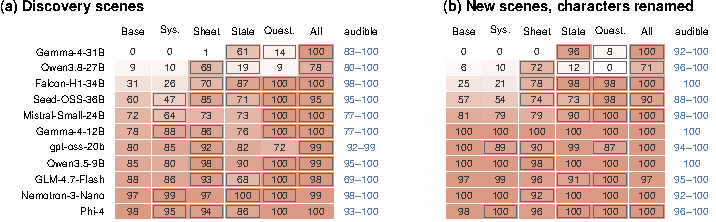
\includegraphics{figures/figB-bridge-all-models.pdf}
\caption{Bridge experiment for all 11 open models. Net use of unheard speech (pp) under Study 2's hearing prompt (Base), with one Study 1 feature swapped in, and with all four. Outlined cells differ from Base with a paired 95\% skeleton-bootstrap interval that excludes zero. The last column gives the range of target use for the same speech when audible (\%). (a) 96 discovery scenes. (b) 96 confirmation scenes with each character renamed to a Study 1 persona.}
\label{fig:bridgefull}
\end{figure}
\begin{table}[!htbp]
\centering\setlength{\tabcolsep}{4.5pt}\small
\begin{tabular}{@{}lrrrrr@{}}
\toprule
\textbf{Model} & \textbf{Study 1 prompt} & \textbf{+ channel} & \textbf{+ question} & \textbf{+ minimal} & \textbf{All three}\\
\midrule
\multicolumn{6}{@{}l}{\emph{Flag: not audible}}\\
Gemma-4-31B & 52.1 & 52.1 & 51.0 & 54.7 & 50.0\\
Qwen3.8-27B & 71.4 & 74.0 & 80.2 & 51.6 & 32.8\\
Seed-OSS-36B & 90.1 & 88.0 & 100.0 & 87.0 & 83.3\\
Phi-4 & 99.0 & 100.0 & 94.3 & 100.0 & 94.3\\
\multicolumn{6}{@{}l}{\emph{Flag: not understood}}\\
Gemma-4-31B & 6.2 & 3.1 & 1.6 & 3.1 & 0.0\\
Qwen3.8-27B & 35.9 & 34.4 & 39.6 & 12.0 & 14.1\\
Seed-OSS-36B & 69.8 & 67.2 & 95.3 & 37.0 & 31.8\\
Phi-4 & 88.5 & 89.6 & 66.1 & 69.8 & 49.5\\
\bottomrule
\end{tabular}
\caption{Format ablation from Study 1 toward Study 2 (96 skeletons, content question): net use (pp) when one Study 2 feature is added (a field naming the channel, the direct question, a minimal context) and with all three.}
\label{tab:ablation}
\end{table}

\end{document}
